% Title: gl2ps_renderer figure
% Creator: GL2PS 1.4.2, (C) 1999-2020 C. Geuzaine
% For: Octave
% CreationDate: Tue Feb 11 08:56:36 2025
\setlength{\unitlength}{1pt}
\begin{picture}(0,0)
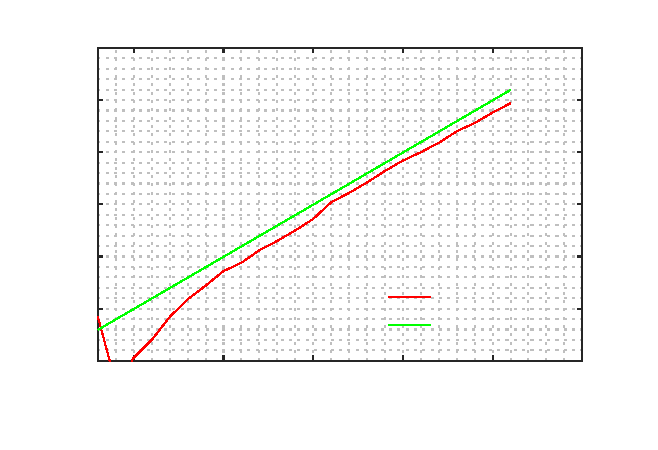
\includegraphics[scale=1]{snr_rx-inc}
\end{picture}%
\begin{picture}(300,200)(0,0)
\fontsize{10}{0}\selectfont\put(56.2222,27){\makebox(0,0)[t]{\textcolor[rgb]{0.15,0.15,0.15}{{-125}}}}
\fontsize{10}{0}\selectfont\put(99.2778,27){\makebox(0,0)[t]{\textcolor[rgb]{0.15,0.15,0.15}{{-120}}}}
\fontsize{10}{0}\selectfont\put(142.333,27){\makebox(0,0)[t]{\textcolor[rgb]{0.15,0.15,0.15}{{-115}}}}
\fontsize{10}{0}\selectfont\put(185.389,27){\makebox(0,0)[t]{\textcolor[rgb]{0.15,0.15,0.15}{{-110}}}}
\fontsize{10}{0}\selectfont\put(228.444,27){\makebox(0,0)[t]{\textcolor[rgb]{0.15,0.15,0.15}{{-105}}}}
\fontsize{10}{0}\selectfont\put(271.5,27){\makebox(0,0)[t]{\textcolor[rgb]{0.15,0.15,0.15}{{-100}}}}
\fontsize{10}{0}\selectfont\put(33.8008,34.8252){\makebox(0,0)[r]{\textcolor[rgb]{0.15,0.15,0.15}{{0}}}}
\fontsize{10}{0}\selectfont\put(33.8008,59.854){\makebox(0,0)[r]{\textcolor[rgb]{0.15,0.15,0.15}{{5}}}}
\fontsize{10}{0}\selectfont\put(33.8008,84.8833){\makebox(0,0)[r]{\textcolor[rgb]{0.15,0.15,0.15}{{10}}}}
\fontsize{10}{0}\selectfont\put(33.8008,109.913){\makebox(0,0)[r]{\textcolor[rgb]{0.15,0.15,0.15}{{15}}}}
\fontsize{10}{0}\selectfont\put(33.8008,134.942){\makebox(0,0)[r]{\textcolor[rgb]{0.15,0.15,0.15}{{20}}}}
\fontsize{10}{0}\selectfont\put(33.8008,159.971){\makebox(0,0)[r]{\textcolor[rgb]{0.15,0.15,0.15}{{25}}}}
\fontsize{10}{0}\selectfont\put(33.8008,185){\makebox(0,0)[r]{\textcolor[rgb]{0.15,0.15,0.15}{{30}}}}
\fontsize{11}{0}\selectfont\put(155.25,13){\makebox(0,0)[t]{\textcolor[rgb]{0.15,0.15,0.15}{{Rx input level (dBm)}}}}
\fontsize{11}{0}\selectfont\put(16.8008,109.913){\rotatebox{90}{\makebox(0,0)[b]{\textcolor[rgb]{0.15,0.15,0.15}{{FM demod output SNR (dB)}}}}}
\fontsize{9}{0}\selectfont\put(202.505,65.3179){\makebox(0,0)[l]{\textcolor[rgb]{0,0,0}{{FM Measured}}}}
\fontsize{9}{0}\selectfont\put(202.505,51.8198){\makebox(0,0)[l]{\textcolor[rgb]{0,0,0}{{FM Theory}}}}
\end{picture}
